\documentclass[tikz,border=7pt]{standalone}
\begin{document}
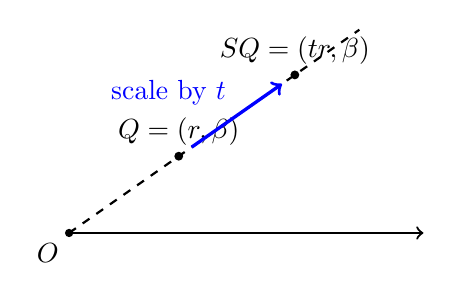
\begin{tikzpicture}[line width=.8pt]
\draw[->] (0,0)--(4.5,0); \draw[dashed] (0,0)--(35:4.5);
\fill (35:1.7) circle (1.6pt) node[above] {$Q=(r,\beta)$};
\fill (35:3.5) circle (1.6pt) node[above] {$S Q=(tr,\beta)$};
\draw[blue,->,very thick] (35:1.9)--(35:3.3) node[midway,above left] {scale by $t$};
\fill (0,0) circle (1.5pt) node[below left] {$O$};
\end{tikzpicture}
\end{document}
